\section{Experiments}\label{sec:experiments}
We compute the constants of Sections~\ref{sec:general}--\ref{sec:population} exactly for trained models. The population $P$ is the held-out empirical law mixed with a uniform mass $\alpha$ over profiles and labels, $\alpha=1\%$ unless stated; it has full support, so $W_\A(P)$ is a local minimax risk. Fixed designs range over all $\binom mb$ forms with the pointwise-unbiased score program of Appendix~\ref{sec:pathdesign}. We report $W_{\rm fixed}/W_{\rm branch}$, the factor by which the best pre-committed design needs more records. \emph{Fitted} designs are optimized on separate reference records and evaluated on $P$.

\begin{figure*}[t]
\centering
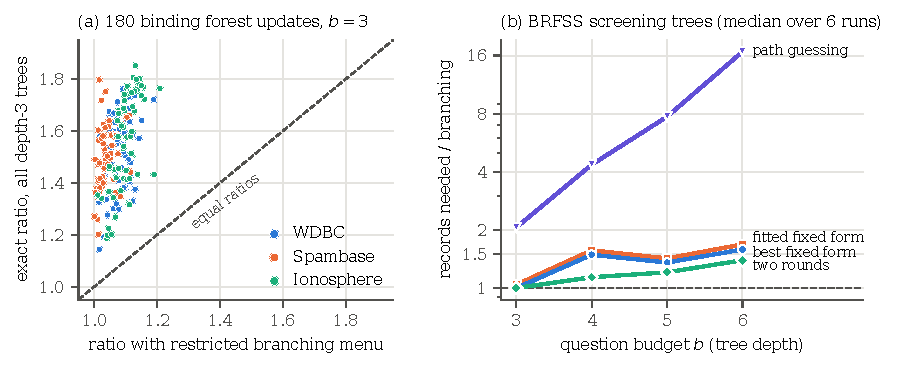
\includegraphics[width=\textwidth]{figures/v12_main.pdf}
\caption{(a) Exact fixed/branching variance ratios for the 180 binding forest updates at cap $b=3$ against the ratio obtained when branching is restricted to the forests' own 40 component trees and all triples. (b) BRFSS screening trees: records needed relative to branching, median over two targets and three seeds.}
\label{fig:v12main}
\end{figure*}

\paragraph{Independently retrained forests.}
On WDBC, Spambase and Ionosphere \citep{wolberg1993,spambase1999,ionosphere1989}, twenty splits each fit an old and a new forest of twenty depth-$b$ trees on disjoint training records, using 3, 6, 9 or 12 median-binarized features. At cap $b=3$ the 180 tasks with more than three candidate features are binding, and column generation over all depth-3 trees converged on every task to certified relative error $10^{-6}$.

\begin{table}[t]
\centering
\caption{Independent forest updates, cap $b=3$, 20 splits per cell. Exact fixed/branching variance ratio over all forms and all depth-3 trees (median and 10th--90th percentiles). Restr.: branching restricted to the 40 component trees and all triples. Fix/full: fixed-form variance relative to the full-information variance. Fitted: designs optimized on training records, evaluated held-out ($m=12$, five splits).}
\label{tab:forestexact}
\footnotesize
\setlength{\tabcolsep}{2.6pt}
\begin{tabular}{llrrrr}
\toprule
Data & $m$ & Exact ratio & Restr. & Fix/full & Fitted \\
\midrule
WDBC & 6 & 1.36 [1.27, 1.48] & 1.08 & 2.11 &  \\
 & 9 & 1.57 [1.43, 1.69] & 1.09 & 3.91 &  \\
 & 12 & 1.66 [1.53, 1.74] & 1.08 & 5.55 & 1.67 \\
Spambase & 6 & 1.41 [1.27, 1.52] & 1.03 & 2.31 &  \\
 & 9 & 1.45 [1.36, 1.59] & 1.03 & 3.09 &  \\
 & 12 & 1.58 [1.49, 1.66] & 1.04 & 4.75 & 1.60 \\
Ionosphere & 6 & 1.36 [1.20, 1.46] & 1.07 & 2.06 &  \\
 & 9 & 1.61 [1.45, 1.77] & 1.10 & 4.19 &  \\
 & 12 & 1.73 [1.58, 1.78] & 1.10 & 5.94 & 1.79 \\
\bottomrule
\end{tabular}
\end{table}


Table~\ref{tab:forestexact} and Figure~\ref{fig:v12main}(a) give three findings. First, adaptivity is worth a median factor 1.51 over the 180 binding tasks (maximum 1.85), and the factor grows with the number of candidate features. Second, a branching menu built from the forests' own component trees captures a median of only 17\% of this gain on the log scale; the optimal designs mix many trees that neither forest contains. Third, even optimal branching stays well above the full-information variance, because forty averaged trees spread the contrast over more coordinates than any three-question path can read.

\paragraph{Cap, dimension and the evaluation law.}
Table~\ref{tab:capgrid} repeats the exact computation for forests of depth $b=2$ and $b=4$ with cap $b$ on five splits per completed cell. Compared with the median 1.51 at $b=3$, at $b=2$ the median over the 45 binding tasks is 1.31 (maximum 1.49, median 1.34 at $m=12$); at $b=4$ the median over the 15 binding tasks is 1.24 (maximum 1.35). Fitted designs realize median ratios within 3\% of the exact ones at every cap ($b=3$: 1.67 against 1.64). Certified column generation at $b=4$ takes about 49 minutes per task at $m=9$, so the $b=4$ cells at $m\ge9$ and $b=5$ were not completed; the two finished WDBC splits at $b=4$, $m=9$ give 1.46 and 1.55 (Appendix~\ref{app:capsens}). The ratios are not artifacts of the smoothing: on the fifteen $m=12$ tasks, changing the uniform mass from 1\% to 0.1\%, 5\% or 10\% changes the exact ratio by a median of 0.8\% and at most 5.3\%, and bootstrap resamples of the held-out records with the forests fixed change it by a median of 1.2\% and at most 7.5\%.

\begin{table}[t]
\centering
\caption{Exact fixed/branching variance ratio for independently retrained depth-$b$ forests with cap $b$ (median over five splits; $b=3$ is in Table~\ref{tab:forestexact}). Cells with $m\le b$ are not binding; cells marked -- were not computed within the compute budget (Appendix~\ref{app:capsens}). Right: number of binding tasks and the median fitted ratio (designs optimized on training records, evaluated held-out).}
\label{tab:capgrid}
\small
\setlength{\tabcolsep}{3.5pt}
\begin{tabular}{lrrrrrr}
\toprule
Data & $b$ & $m=6$ & $m=9$ & $m=12$ & tasks & fitted \\
\midrule
WDBC & 2 & 1.31 & 1.23 & 1.27 & 45 & 1.31 \\
Spambase & & 1.35 & 1.25 & 1.35 & & \\
Ionosphere & & 1.31 & 1.44 & 1.42 & & \\
\addlinespace[1pt]
WDBC & 4 & 1.23 & -- & -- & 15 & 1.26 \\
Spambase & & 1.28 & -- & -- & & \\
Ionosphere & & 1.20 & -- & -- & & \\
\addlinespace[1pt]
\bottomrule
\end{tabular}
\end{table}


\paragraph{Budgeted screening questionnaires.}
A depth-$b$ screening tree asks at most $b$ questions per person, so a validation study under the same burden must also respect the cap. We train class-balanced CART trees of depth $b\in\{3,4,5,6\}$ on two datasets. The CDC Diabetes Health Indicators data, derived from the Behavioral Risk Factor Surveillance System \citep{cdcdiabetes2017}, provide twelve yes/no survey items for 253,680 respondents and the target diabetes or prediabetes. The thyroid data provide twelve binarized history and laboratory items for 7,200 patients and an abnormal-function target \citep{quinlan1986thyroid}, a standard benchmark for cost-sensitive test ordering \citep{turney1995}. Trees are trained on source records and validated on a target (a disjoint random half, or respondents of the other sex); the estimand is the target accuracy of the tree's deterministic decision, and branching asks the tree's own questions, attaining the full-information variance.

\begin{table}[t]
\centering
\caption{Budgeted screening trees: records needed relative to branching (which asks the tree's own questions), median over two targets (random half, other sex) and three seeds. Best: optimal fixed-form design for the target law; Fitted: designed on source records; Guess: uniform path guessing; Two: follow the root question, then the best fixed form. Lower, Upper: medians of the two ends of the variance-scale bracket of Theorem~\ref{thm:bracket}, computed at the target law.}
\label{tab:screening}
\small
\setlength{\tabcolsep}{3.2pt}
\begin{tabular}{lrrrrrr}
\toprule
Data, $b$ & Best & Fitted & Guess & Two & Lower & Upper \\
\midrule
BRFSS, 3 & 1.00 & 1.04 & 2.1 & 1.00 & 1.00 & 1.5 \\
BRFSS, 4 & 1.49 & 1.57 & 4.4 & 1.14 & 1.18 & 3.6 \\
BRFSS, 5 & 1.35 & 1.42 & 7.7 & 1.21 & 1.08 & 5.9 \\
BRFSS, 6 & 1.58 & 1.68 & 16.7 & 1.39 & 1.13 & 11.4 \\
Thyroid, 3 & 1.00 & 1.04 & 4.4 & 1.00 & 1.00 & 3.5 \\
Thyroid, 4 & 1.00 & 1.04 & 6.7 & 1.00 & 1.00 & 4.9 \\
Thyroid, 5 & 1.00 & 1.04 & 9.2 & 1.00 & 1.00 & 6.1 \\
Thyroid, 6 & 1.00 & 1.03 & 10.5 & 1.00 & 1.00 & 6.5 \\
\bottomrule
\end{tabular}
\end{table}


Table~\ref{tab:screening} and Figure~\ref{fig:v12main}(b) show that the gain depends on how many questions the screening decision needs. On BRFSS the best pre-committed design needs a median of 1.35--1.58 times as many respondents for $b=4,5,6$, and up to 1.98 times in a single run. On thyroid, every thresholded tree, up to depth six, depends on at most $b$ items. Then $\Gamma_P=1$, the best fixed form computes the decision, and pre-commitment costs nothing intrinsic. The bracket detects this from reference data before any collection. Completion-only path guessing, the estimator behind the classical simulation of a tree by fixed queries, needs up to 25 times as many respondents; optimized fixed-form scores remove most of this cost and leave only the intrinsic part. That part accrues over rounds: following the root question and then using the best fixed form, a feasible but not optimal two-round design, recovers a median 33--63\% of the log-gap depending on the cap, and three rounds recover 57--100\%. Fitted designs lose 3--7\% relative to their oracles. Every run lies inside the variance-scale bracket of Theorem~\ref{thm:bracket} up to the solver tolerance of $10^{-8}$, and the lower end is the closer bound. Computed from reference records alone, the lower end of the bracket predicts the realized ratio with Spearman correlation 0.78 over the 48 screening runs and never exceeds it; all 31 runs with a reference lower end at most 1.05 realize a gain of at most 1.25. For the 240 forest tasks, where no single tree computes the contrast, the correlation is 0.52 and the realized ratio falls below the reference-law value in 75 tasks (Appendix~\ref{app:capsens}).

\paragraph{Information versus design.}
Multiple imputation from complete source records uses information the capped audit does not collect. In simulated audits of 1,000 respondents (Appendix~\ref{app:screening}), its RMSE is 0.88--1.00 times that of branching with coverage 0.94--0.99 under both targets, because the conditional law of unasked items transports here. A model-assisted estimator that imputes the conditional mean of the target from the same source records, without any imputation draws, attains RMSE 0.89--0.99 times that of branching with coverage 0.94--0.96 in the same audits (Appendix~\ref{app:regimp}): information, not design, closes the gap. The design-based scores need neither the reference nor the transport assumption, and their RMSE is 1.00--1.22 times that of branching; the practical case for within-record adaptivity is the setting without a trusted complete reference.

\paragraph{A real planned-missing archive.}
PISA 2012 assigned three questionnaire forms at random, and no U.S. student answered all nine predictors of our block-averaged forest ensembles; every block pair appears on a form, so the Brier contrast is identifiable from the actual menu, and optimized form scores, a block/pair Horvitz--Thompson score and multiple imputation agree, with all intervals including zero (Appendix~\ref{app:pisa}). The archive demonstrates identification from real fixed forms and has no branching counterfactual.
